\documentclass[10pt]{article}
\usepackage{fullpage}
\usepackage{graphicx}
\usepackage{caption}
\usepackage{url}
\usepackage{longtable}
\usepackage{colortbl}
\usepackage{color}
\usepackage{lscape}

\newcommand{\chidb}{$\chi$\textsf{db}}

%opening
\title{The \chidb{} Architecture\\{\large Version 0.20100327}}
\author{Borja Sotomayor}
\date{}

\begin{document}
\pagestyle{empty}
\maketitle

\chidb{} is a didactic relational database management system (RDBMS) designed for teaching how a RDBMS is built internally, from the data organization in files all the way up to the SQL parser and query optimizer. The design of \chidb{} is based on SQLite\footnote{\url{http://www.sqlite.org/}}, with several simplifying assumptions that make it possible to develop a complete \chidb{} implementation over the course of a quarter or semester. One of the key similarities is that \chidb{} uses a single file to store all its information (database metadata, tables, and indexes). In fact, the \chidb{} file format is a subset of SQLite, meaning that well-formed \chidb{} files will also be well-formed SQLite files (the opposite, though, is not necessarily true).

This document describes the architecture of the \chidb{} RDBMS. We assume a basic knowledge of RDBMS, particularly tables, records, keys, indexes, and SQL. The \chidb{} architecture, summarized in Figure~\ref{fig:arch} is divided into three broad areas:



\begin{figure}
\begin{center}
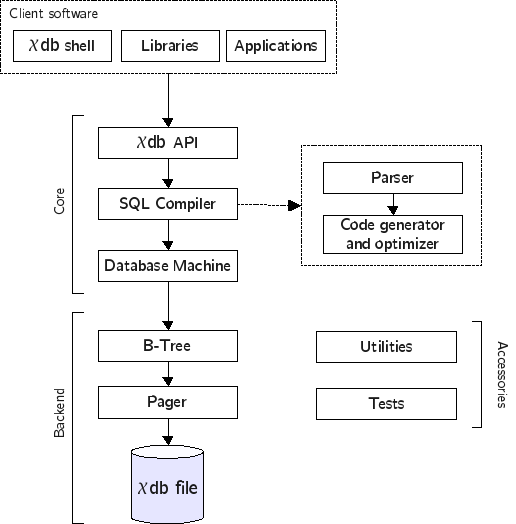
\includegraphics[width=0.5\textwidth]{images/arch_overview.png}
\caption{\chidb{} architecture}
\end{center}
\label{fig:arch}
\end{figure}


\begin{description}
\item[Backend] Contains the \emph{\textbf{B-Tree module}} and the \emph{\textbf{Pager module}}. The B-Tree module is responsible for managing a collection of file-based B-Trees, using the \chidb{} file format. However, the B-Tree module does not include any I/O code. All I/O is delegated to the Pager, which provides a page-by-page access to a \chidb{} file. The Pager may include a page cache to optimize disk access.

The specifications of the \chidb{} file format is outside the scope of this document (but can be found on a separate document, \emph{The \chidb{} File Format}).

\item[Core] Contains the \emph{\textbf{\chidb{} API}}, a \emph{\textbf{SQL compiler}}, and a \emph{\textbf{database machine}} (or DBM). The API is the interface that other applications must go through to use a \chidb{} file, and allows client software to open a \chidb{} file, execute SQL statements on that file, and close the file. When a SQL statement is submitted, it is processed by the SQL compiler. The compiler itself is divided into two modules: a SQL parser, which produces a convenient in-memory representation of a SQL query, and the code generator and optimizer, which generates code for the database machine. The database machine is a virtual machine specifically designed to operate on \chidb{} files, and includes instructions such as ``Create a new table'', ``Find a record with key $k$'', etc.

Section~\ref{sec:api} specifies the \chidb{} API, Section~\ref{sec:sql} specifies the subset of SQL supported by \chidb{}, and Section~\ref{sec:dbm} specifies the architecture of the \chidb{} DBM and its instructions. How to generate DBM code based on a given SQL statement is outside the scope of this document.

\item[Accessories] Includes a \emph{\textbf{utilities}} modules, with miscellaneous code that are used across all modules, and \emph{\textbf{testing}} code.
\end{description}


\section{\chidb{} API}
\label{sec:api}

The \chidb{} API comprises a set of functions that allows client software to access and manipulate \chidb{} files, including executing SQL statements on them. Unless otherwise noted, each API function returns one of the return codes listed in Table~\ref{tab:codes} (this table lists every possible return code; the description of each API function notes what return codes can be returned by that specific function). This document describes a C API. Bindings with other languages must provide equivalent functionality to the API described here.

\begin{table}
\caption{API return codes}
\begin{center}
\sffamily
\begin{tabular}{|l|l|l|}
\hline \textbf{Name} & \textbf{Integer code} & \textbf{Description} \\ \hline\hline
\verb+CHIDB_OK+ & 0 & Succesful result \\ \hline
\verb+CHIDB_EINVALIDSQL+ & 1 & Invalid SQL \\ \hline
\verb+CHIDB_ENOMEM+ & 2 & Could not allocate memory \\ \hline
\verb+CHIDB_ECANTOPEN+ & 3 & Unable to open the database file\\ \hline
\verb+CHIDB_ECORRUPT+ & 4 & The database file is not well formed \\ \hline
\verb+CHIDB_ECONSTRAINT+ & 5 & SQL statement failed because of a constraint violation\\ \hline
\verb+CHIDB_EMISMATCH+ & 6 & Data type mismatch\\ \hline
\verb+CHIDB_EIO+ & 7 & An I/O error has occurred when accessing the file \\ \hline
\verb+CHIDB_EMISUSE+ & 8 & API used incorrectly\\ \hline
\verb+CHIDB_ROW+ & 100 & \verb+chidb_step()+ has another row ready\\ \hline
\verb+CHIDB_DONE+ & 101 & \verb+chidb_step()+ has finished executing\\ \hline
\end{tabular}
\end{center}
\label{tab:codes}
\end{table}

\subsection{\texttt{chidb\_open}}

The \verb+chidb_open+ function is used to open a \chidb{} file. Its signature is the following:

\begin{verbatim}
int chidb_open(
  const char* file, 
  chidb**     db
);
\end{verbatim}

\texttt{file} is the filename of the \chidb{} file to open. If the file does not exist, it will be created. \texttt{db} is used to return a pointer to a \texttt{chidb} variable. The \texttt{chidb} type is an \emph{opaque} type representing a \chidb{} database. In other words, an API user should not be concerned with what is contained in a \texttt{chidb} variable, and should simply use it as a representation of a \chidb{} database to pass along to other API functions.

The return value of the function can be \verb+CHIDB_OK+, \verb+CHIDB_ENOMEM+, \verb+CHIDB_ECANTOPEN+, \verb+CHIDB_ECORRUPT+, or \verb+CHIDB_EIO+.

\subsection{\texttt{chidb\_close}}

The \verb+chidb_close+ function is used to close a \chidb{} file. Its signature is the following:

\begin{verbatim}
int chidb_close(chidb *db); 
\end{verbatim}

\texttt{db} is the database to close.

The return value of the function can be \verb+CHIDB_OK+ or \verb+CHIDB_EMISUSE+ (if called on a database that is already closed).


\subsection{\texttt{int chidb\_prepare}}

The \verb+chidb_prepare+ function is used to prepare a SQL statement for execution. Internally, this will require compiling the SQL statement (but not running it yet). The function's signature is:

\begin{verbatim}
int chidb_prepare(
  chidb*       db, 
  const char*  sql, 
  chidb_stmt** stmt
);
\end{verbatim}

\texttt{db} is the database on which to run the SQL statement. \texttt{sql} is the SQL statement itself. \texttt{stmt} is used to return a pointer to a \verb+chidb_stmt+ variable. The \verb+chidb_stmt+ type is an \emph{opaque} type representing a SQL statement.

The return value of the function can be \verb+CHIDB_OK+, \verb+CHIDB_EINVALIDSQL+, \verb+CHIDB_ENOMEM+.

\subsection{\texttt{int chidb\_step}}

The \verb+chidb_step+ function runs a prepared SQL statement until a result row is available (or just runs the SQL statement to completion if it is not meant to produce a result row, such as an INSERT statement). Its signature is: 

\begin{verbatim}
int chidb_step(chidb_stmt *stmt);
\end{verbatim}

\texttt{stmt} is the SQL statement to run.

If the statement is a SELECT statement, \verb+chidb_step+ returns \verb+CHIDB_ROW+ each time a result row is produced. The values of the result row can be accessed using the column access functions described below. Thus, \verb+chidb_step+ has to be called repeatedly to access all the rows returned by the query. Once there are no more rows left, or if the statement is not meant to produce any results, then \verb+CHIDB_DONE+ is returned (note that this function does not return \verb+CHIDB_OK+).

The function can also return \verb+CHIDB_ECONSTRAINT+, \verb+CHIDB_EMISMATCH+, \verb+CHIDB_EMISUSE+ (if called on a finalized SQL statement), or \verb+CHIDB_EIO+.

\subsection{\texttt{int chidb\_finalize}}

The \verb+chidb_finalize+ function finalizes a SQL statement, freeing all resources associated with it.

\begin{verbatim}
int chidb_finalize(chidb_stmt *stmt);
\end{verbatim}

\texttt{stmt} is the SQL statement to finalize.

The return value of the function can be \verb+CHIDB_OK+ or \verb+CHIDB_EMISUSE+ (if called on a statement that is already finalized).


\subsection{Column access functions}

Once a SQL statement has been prepared, the following three functions can be used to obtain information on the columns of the rows that will be returned by the statement:

\begin{verbatim}
int chidb_column_count(chidb_stmt *stmt);

int chidb_column_type(
  chidb_stmt* stmt, 
  int         col
);

const char *chidb_column_name(
  chidb_stmt* stmt, 
  int         col
);
\end{verbatim}

In all these functions, the \texttt{stmt} parameter is the prepared SQL statement.

\verb+chidb_column_count+ returns the number of columns in the result rows. If the SQL statement is not meant to produce any results (such as an INSERT statement), then 0 is returned.

\verb+chidb_column_type+ returns the type of column \texttt{col} (columns are numbered from 0). The supported types are summarized in Table~\ref{tab:sqltypes}.

\verb+chidb_column_name+ returns a pointer to a null-terminated string containing the name of column \texttt{col}. The API client does not have to \texttt{free()} the returned string. It is the API function's responsibility to allocate and free the memory for this string. 

\begin{table}
\caption{SQL types}
\begin{center}
\sffamily
\begin{tabular}{|c|c|c|p{7cm}|}
\hline \textbf{Integer code} & \textbf{SQL type} & \textbf{Description} \\ \hline\hline
0 & \texttt{NULL} & Null value.  \\ \hline
1 & \texttt{BYTE} & 1-byte signed integer. \\ \hline
2 & \texttt{SMALLINT} & 2-byte signed integer. \\ \hline
4 & \texttt{INTEGER} & 4-byte signed integer. \\ \hline
13 & \texttt{TEXT} & Character string. \\ \hline
\end{tabular}
\end{center}
\label{tab:sqltypes}
\end{table}

If \verb+chidb_step+ returns \verb+CHIDB_ROW+, the following two functions can be used to access the contents of each column:

\begin{verbatim}
int chidb_column_int(
  chidb_stmt* stmt, 
  int         col
);

const char *chidb_column_text(
  chidb_stmt* stmt, 
  int         col
);
\end{verbatim}

In all these functions, the \texttt{stmt} parameter is the SQL statement.

\verb+chidb_column_int+ returns the integer value in column \texttt{col} of the row. The column must be of type \texttt{BYTE}, \texttt{SMALLINT}, or \texttt{INTEGER}.

\verb+chidb_column_text+ returns a pointer to a null-terminated string containing the value in column \texttt{col} of the row. The API client does not have to \texttt{free()} the returned string. It is the API function's responsibility to allocate and free the memory for this string. 


Note that none of these functions return error codes. Calling the column access functions on an unprepared statement, or accessing column values on a statement that has not produced a result row, will produce unexpected behaviour.

\section{Supported SQL}
\label{sec:sql}

\begin{figure}
\input{sql_grammar}
\caption{Grammar for subset of SQL supporter by \chidb. Literal tokens as shown in \textbf{``DOUBLE-QUOTED UPPERCASE BOLD''}. Token TK\_ID represents an identifier (an alphanumeric string starting with a letter and at least one character), TK\_INT represents an integer, and TK\_STRING represents a double-quoted string.}
\label{fig:sql}
\end{figure}

\chidb{} supports a very limited subset of the SQL language. However, this subset is still sufficiently featureful to run basic queries and perform interesting query optimizations. The exact grammar is shown in Figure~\ref{fig:sql}, and has the following main constraints:

\begin{enumerate}
\item The field list in a SELECT statement can only be a list of columns in the form ``[table.]column'' or ``*''. Subqueries, arithmetic expressions, and aggregate functions are not supported.
\item The FROM clause can only be a list of table names. The AS operator is not supported.
\item The WHERE clause can only be a list of AND'ed conditions (e.g., \emph{cond1} AND \emph{cond2} \ldots AND \emph{condN}). Each condition can only be of the form ``column operator value'' or ``column operator column''. Only the $=$, $<>$, $>$, $<$, $>=$, $<=$, IS NULL, and IS NOT NULL operators are supported.
\item The VALUES clause of an INSERT operator must always provide literal integer or string values. Subqueries or arithmetic operations are not supported.
\item In accordance with the \chidb{} file format, CREATE TABLE can only create tables with BYTE, SMALLINT, INTEGER, or TEXT columns. The primary key can only be an INTEGER field.
\item In accordance with the \chidb{} file format, CREATE INDEX can only create indexes on a single integer field.
\end{enumerate}

\section{Database Machine}
\label{sec:dbm}

\begin{figure}
\begin{center}
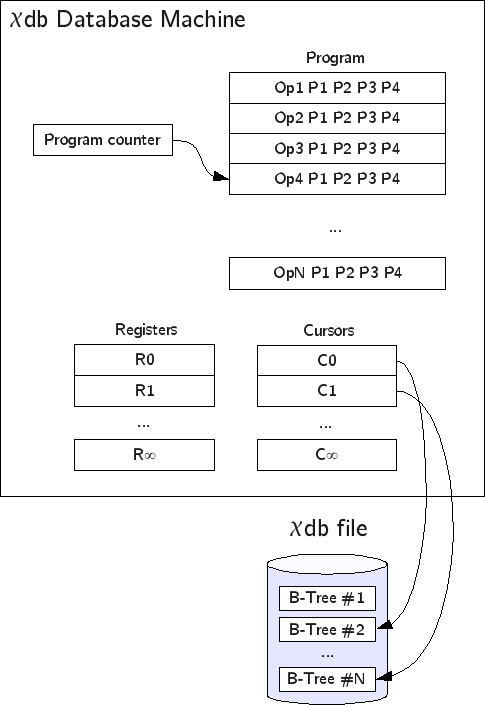
\includegraphics[width=0.4\textwidth]{images/dbm.png}
\caption{\chidb{} Database Machine}
\end{center}
\label{fig:dbm}
\end{figure}

The database machine (or DBM) is a computing machine specifically designed to operate on \chidb{} files, and includes instructions such as ``Create a new table'', ``Find a record with key $k$'', etc. The DBM architecture, summarized in Figure~\ref{fig:dbm}, includes the following components:

\begin{description}
\item[The DBM program] A DBM program is composed of one or more DBM instructions. An instruction contains an operator code and up to four operands: P1, P2, P3, and P4. P1 through P3 are signed 32-bit integers, and P4 is a pointer to a null-terminated string. All the DBM instructions are listed in Table~\ref{tab:dbmops}. Instructions in the DBM program are numbered from 0.
\item[Program counter] Keeps track of what instruction is currently being executed. Certain instructions can directly modify the program counter to jump to a specific instruction in the program.
\item[Registers] The DBM has an unlimited number of registers. A register can contain a 32-bit signed integer, a pointer to a null-terminated string or to raw binary data, or a NULL value. Registers are numbered from 0.
\item[Cursors] A cursor is a pointer to a specific entry in a B-Tree. Cursors must be able to move to the next or previous entry in a B-Tree in $O(1)$ time.
\end{description}

A DBM starts executing a program on the $0^{\textrm{th}}$ instruction, and executes  subsequent instructions sequentially until a \texttt{Halt} instruction is encountered, or until the program counter advances past the end of the program (which is equivalent to a \texttt{Halt} instruction with all its parameters set to 0). Note that it is also possible for individual instructions to fail, resulting in a premature termination of the program.


\begin{landscape}
\begin{longtable}{|c|p{3cm}|p{3cm}|p{3cm}|p{3cm}|p{4cm}|}
\caption{\chidb{} DBM instructions} \label{tab:dbmops} \\


\hline \textbf{Instruction} & \textbf{P1} & \textbf{P2}  & \textbf{P3}  & \textbf{P4}  & \textbf{Description}\\ \hline 
\endfirsthead

\multicolumn{6}{c}{{\bfseries \tablename\ \thetable{} -- continued from previous page}} \\
\hline \textbf{Instruction} & \textbf{P1} & \textbf{P2}  & \textbf{P3}  & \textbf{P4}  & \textbf{Description}\\ \hline 
\endhead

\multicolumn{6}{r}{\emph{Continued on next page\ldots}} \\
\endfoot

\hline \hline
\endlastfoot


%%%%%%%%%%%%%%%%%%%%%%%%%%%%%%%%%%%%%%%%%%%%%%%%%%%%%%%%%%%%%%%%%%
%
%     Table opening
%
%%%%%%%%%%%%%%%%%%%%%%%%%%%%%%%%%%%%%%%%%%%%%%%%%%%%%%%%%%%%%%%%%%

\texttt{OpenRead} & 
A cursor $c$ & 
A register $r$. The register must contain a page number $n$ & 
The number of columns in the table (0 if opening an index) &
\cellcolor[gray]{0.9} &
Opens the B-Tree rooted at the page $n$ for read-only access and stores a cursor for it in $c$. \\\hline

\texttt{OpenWrite} & 
\multicolumn{5}{c|}{Same as \texttt{OpenRead}, but opening the B-Tree in read/write mode.} \\\hline

\texttt{Close} & 
A cursor $c$ & 
\cellcolor[gray]{0.9} & 
\cellcolor[gray]{0.9} &
\cellcolor[gray]{0.9} &
Closes cursor $c$ and frees up any resources associated with it. \\\hline


%%%%%%%%%%%%%%%%%%%%%%%%%%%%%%%%%%%%%%%%%%%%%%%%%%%%%%%%%%%%%%%%%%
%
%     Cursor movement
%
%%%%%%%%%%%%%%%%%%%%%%%%%%%%%%%%%%%%%%%%%%%%%%%%%%%%%%%%%%%%%%%%%%

\texttt{Rewind} & 
A cursor $c$ & 
A jump address $j$ & 
\cellcolor[gray]{0.9} &
\cellcolor[gray]{0.9} &
Makes cursor $c$ point to the first entry in the B-Tree. If the B-Tree is empty, then jump to $j$. \\\hline

\texttt{Next} & 
A cursor $c$ & 
A jump address $j$ & 
\cellcolor[gray]{0.9} &
\cellcolor[gray]{0.9} &
Advance cursor $c$ to the next entry in the B-Tree and jump to $j$. If there are no more entries (if cursor $c$ was pointing at the last entry in the B-Tree), do nothing. \\\hline

\texttt{Prev} & 
\multicolumn{5}{c|}{Same as \texttt{Next}, but moving the cursor to the previous entry.} \\\hline

\texttt{Seek} & 
A cursor $c$ & 
A jump address $j$ & 
A key $k$ &
\cellcolor[gray]{0.9} &
Move cursor $c$ to point to the entry with key equal to $k$. If the B-Tree doesn't contain such an entry, jump to $j$. \\\hline

\texttt{SeekGt} & 
A cursor $c$ & 
A jump address $j$ & 
A register $r$. The register must contain a key $k$. &
\cellcolor[gray]{0.9} &
Move cursor $c$ to the first entry such that its key is greater than $k$. If there is no such entry, jump to $j$. \\\hline

\texttt{SeekGe} & 
\multicolumn{5}{c|}{Same as \texttt{SeekGt}, but moving the cursor to the first entry such that its key is greater than or equal to $k$.} \\\hline

%%%%%%%%%%%%%%%%%%%%%%%%%%%%%%%%%%%%%%%%%%%%%%%%%%%%%%%%%%%%%%%%%%
%
%     Cursor access
%
%%%%%%%%%%%%%%%%%%%%%%%%%%%%%%%%%%%%%%%%%%%%%%%%%%%%%%%%%%%%%%%%%%

\texttt{Column} & 
A cursor $c$ & 
A column number $n$.& 
A register $r$ &
\cellcolor[gray]{0.9} &
Store in register $r$ the value in the $n$-th column of the entry pointed at by cursor $c$. Columns are numbered from 0. \\\hline

\texttt{Key} & 
A cursor $c$ & 
A register $r$ &
\cellcolor[gray]{0.9} &
\cellcolor[gray]{0.9} &
Store in register $r$ the value of the key of the entry pointed at by cursor $c$.\\\hline

%%%%%%%%%%%%%%%%%%%%%%%%%%%%%%%%%%%%%%%%%%%%%%%%%%%%%%%%%%%%%%%%%%
%
%     Register manipulation
%
%%%%%%%%%%%%%%%%%%%%%%%%%%%%%%%%%%%%%%%%%%%%%%%%%%%%%%%%%%%%%%%%%%

\texttt{Integer} & 
An integer $i$ & 
A register $r$ &
\cellcolor[gray]{0.9} &
\cellcolor[gray]{0.9} &
Store $i$ in $r$.\\\hline

\texttt{String} & 
A length $l$ & 
A register $r$ &
\cellcolor[gray]{0.9} &
A string $s$ &
Store $s$ (with length $l$) in $r$.\\\hline

\texttt{Null} & 
\cellcolor[gray]{0.9} & 
A register $r$ &
\cellcolor[gray]{0.9} &
\cellcolor[gray]{0.9} &
Store a null value in $r$.\\\hline


%%%%%%%%%%%%%%%%%%%%%%%%%%%%%%%%%%%%%%%%%%%%%%%%%%%%%%%%%%%%%%%%%%
%
%     Record manipulation
%
%%%%%%%%%%%%%%%%%%%%%%%%%%%%%%%%%%%%%%%%%%%%%%%%%%%%%%%%%%%%%%%%%%

\texttt{ResultRow} & 
A register $r$ & 
An integer $n$ &
\cellcolor[gray]{0.9} &
\cellcolor[gray]{0.9} &
This instructions indicates that a result row has been produced and pauses execution for the database machine user to fetch the result row. The result row is formed by the values stored in registers $r$ through $r+n-1$.\\\hline

\texttt{MakeRecord} & 
A register $r_1$& 
An integer $n$ &
A register $r_2$ &
\cellcolor[gray]{0.9} &
Create a database record using the values from registers $r_1$ through $r_1+n-1$, and store the record in $r_2$.\\\hline

%%%%%%%%%%%%%%%%%%%%%%%%%%%%%%%%%%%%%%%%%%%%%%%%%%%%%%%%%%%%%%%%%%
%
%     Insertion
%
%%%%%%%%%%%%%%%%%%%%%%%%%%%%%%%%%%%%%%%%%%%%%%%%%%%%%%%%%%%%%%%%%%

\texttt{Insert} & 
A cursor $c$ & 
A register $r_1$. The register must contain a database record $v$. &
A register $r_2$. The register must contain a key $k$. &
\cellcolor[gray]{0.9} &
Inserts an entry, with key $k$ and value $v$, in the B-Tree pointed at by cursor $c$.\\\hline

%%%%%%%%%%%%%%%%%%%%%%%%%%%%%%%%%%%%%%%%%%%%%%%%%%%%%%%%%%%%%%%%%%
%
%     Conditional Statements
%
%%%%%%%%%%%%%%%%%%%%%%%%%%%%%%%%%%%%%%%%%%%%%%%%%%%%%%%%%%%%%%%%%%

\texttt{Eq} & 
A register $r_1$ & 
A jump address $j$ &
A register $r_2$ &
\cellcolor[gray]{0.9} &
If the contents of $r_1$ are equal to the contents of $r_2$, jump to $j$. Otherwise, do nothing. This instruction assumes that the types of the contents of both registers are the same.\\\hline

\texttt{Ne} & 
\multicolumn{5}{c|}{Same at \texttt{Eq}, but testing for inequality of values.} \\\hline

\texttt{Lt} & 
\multicolumn{5}{c|}{Same at \texttt{Eq}, but testing for the value in $r_1$ being less than the value in $r_2$.} \\\hline

\texttt{Le} & 
\multicolumn{5}{c|}{Same at \texttt{Eq}, but testing for the value in $r_1$ being less than or equal to the value in $r_2$.} \\\hline

\texttt{Gt} & 
\multicolumn{5}{c|}{Same at \texttt{Eq}, but testing for the value in $r_1$ being greater than the value in $r_2$.} \\\hline

\texttt{Ge} & 
\multicolumn{5}{c|}{Same at \texttt{Eq}, but testing for the value in $r_1$ being greater than or equal to the value in $r_2$.} \\\hline

%%%%%%%%%%%%%%%%%%%%%%%%%%%%%%%%%%%%%%%%%%%%%%%%%%%%%%%%%%%%%%%%%%
%
%     Index Manipulation
%
%%%%%%%%%%%%%%%%%%%%%%%%%%%%%%%%%%%%%%%%%%%%%%%%%%%%%%%%%%%%%%%%%%

\texttt{IdxGt} & 
A cursor $c$ & 
A jump address $j$ &
A register $r$. Must contain a key $k$. &
\cellcolor[gray]{0.9} &
Cursor $c$ points to an index entry containing a $(\textsc{IdxKey},\textsc{PKey})$ pair. If \textsc{PKey} is greater than $k$, jump to $j$. Otherwise, do nothing.\\\hline

\texttt{IdxGe} & 
\multicolumn{5}{c|}{Same as \texttt{IdxGt}, but testing for \textsc{PKey} being greater than or equal to $k$.} \\\hline

\texttt{IdxLt} & 
\multicolumn{5}{c|}{Same as \texttt{IdxGt}, but testing for \textsc{PKey} being less than $k$.} \\\hline

\texttt{IdxLe} & 
\multicolumn{5}{c|}{Same as \texttt{IdxGt}, but testing for \textsc{PKey} being less than or equal to $k$.} \\\hline

\texttt{IdxKey} & 
A cursor $c$ & 
A register $r$ &
\cellcolor[gray]{0.9} &
\cellcolor[gray]{0.9} &
Cursor $c$ points to an index entry containing a $(\textsc{IdxKey},\textsc{PKey})$ pair. Store \textsc{PKey} in $r$.\\\hline

\texttt{IdxInsert} & 
A cursor $c$ & 
A register $r_1$, containing a key \textsc{IdxKey} &
A register $r_2$, containing a key \textsc{PKey} &
\cellcolor[gray]{0.9} &
Add a new $(\textsc{IdxKey},\textsc{PKey})$ entry in the index B-Tree pointed at by cursor $c$.\\\hline

%%%%%%%%%%%%%%%%%%%%%%%%%%%%%%%%%%%%%%%%%%%%%%%%%%%%%%%%%%%%%%%%%%
%
%     Create
%
%%%%%%%%%%%%%%%%%%%%%%%%%%%%%%%%%%%%%%%%%%%%%%%%%%%%%%%%%%%%%%%%%%

\texttt{CreateTable} & 
A register $r$. & 
\cellcolor[gray]{0.9} &
\cellcolor[gray]{0.9} &
\cellcolor[gray]{0.9} &
Create a new table B-Tree and store its root page in $r$.\\\hline

\texttt{CreateIndex} & 
\multicolumn{5}{c|}{Same as \texttt{CreateTable}, but creating an index B-Tree.} \\\hline

%%%%%%%%%%%%%%%%%%%%%%%%%%%%%%%%%%%%%%%%%%%%%%%%%%%%%%%%%%%%%%%%%%
%
%     Misc
%
%%%%%%%%%%%%%%%%%%%%%%%%%%%%%%%%%%%%%%%%%%%%%%%%%%%%%%%%%%%%%%%%%%

\texttt{SCopy} & 
A register $r_1$ & 
A register $r_2$ &
\cellcolor[gray]{0.9} &
\cellcolor[gray]{0.9} &
Make a shallow copy of the contents of $r_1$ into $r_2$. In other words, $r_2$ must be left pointing to the same value as $r_1$.\\\hline

\texttt{Halt} & 
An integer $n$ & 
\cellcolor[gray]{0.9}&
\cellcolor[gray]{0.9} &
An error message $s$  &
Halt execution of the database machine and return error code $n$. If $n!=0$, set the machine's error message to $s$.\\\hline

\end{longtable}
\end{landscape}


\section{Copyright information}

This work is licensed under the Creative Commons Attribution-Share Alike 3.0 United States License. To view a copy of this license, visit http://creativecommons.org/licenses/by-sa/3.0/us/ or send a letter to Creative Commons, 171 Second Street, Suite 300, San Francisco, California, 94105, USA.


\end{document}
